\documentclass[border=4pt]{standalone}
% Shared style for FORGE paper figures (standalone, vector PDF)
\usepackage[T1]{fontenc}
\usepackage{lmodern}      % Latin Modern sans serif for diagrams
\renewcommand{\familydefault}{\sfdefault}
\usepackage{microtype}
\DisableLigatures[-]{encoding=T1,family=tt*}  % keep -- as two hyphens in CLI flags
\usepackage{textcomp}
\usepackage{amsmath}
\usepackage{tikz}
\usetikzlibrary{arrows.meta,positioning,calc,fit,backgrounds,shapes.geometric,shapes.misc,decorations.pathreplacing}

% ---- Moderate accent palette -------------------------------------------------
\definecolor{ink}{HTML}{222831}        % near-black text/borders
\definecolor{subink}{HTML}{5B6470}     % secondary text
\definecolor{accInput}{HTML}{2F5C9E}   % blue  -> plugin inputs
\definecolor{accModel}{HTML}{2A9D8F}   % teal  -> validated model / core
\definecolor{accGen}{HTML}{D7892B}     % amber -> generators / outputs
\definecolor{accVerif}{HTML}{6A4C93}   % purple-> verification
\definecolor{accMuted}{HTML}{8A94A3}   % grey  -> not-exercised / external

\colorlet{fillInput}{accInput!10}
\colorlet{fillModel}{accModel!14}
\colorlet{fillGen}{accGen!14}
\colorlet{fillVerif}{accVerif!12}
\colorlet{fillMuted}{accMuted!14}
\colorlet{fillPlain}{black!4}

% ---- Node styles -------------------------------------------------------------
\tikzset{
  font=\sffamily,
  >={Stealth[length=2.6mm,width=2.0mm]},
  base/.style={
    rounded corners=2pt, draw, line width=0.7pt,
    align=center, inner sep=5pt, text=ink,
    minimum height=10mm, font=\small},
  inbox/.style   ={base, draw=accInput, fill=fillInput},
  modelbox/.style={base, draw=accModel, fill=fillModel, line width=1.0pt},
  genbox/.style  ={base, draw=accGen,   fill=fillGen},
  verbox/.style  ={base, draw=accVerif, fill=fillVerif},
  mutedbox/.style={base, draw=accMuted, fill=fillMuted, text=subink},
  outbox/.style  ={base, draw=ink!55,   fill=fillPlain},
  title/.style   ={font=\bfseries\small, text=ink},
  grouptitle/.style={font=\bfseries\footnotesize, text=#1},
  lbl/.style     ={font=\scriptsize, text=subink, inner sep=2pt},
  flow/.style    ={draw=ink!70, line width=0.9pt, ->},
  flowmuted/.style={draw=accMuted, line width=0.8pt, ->, densely dashed},
  flowmodel/.style={draw=accModel, line width=1.1pt, ->},
  groupbg/.style ={rounded corners=4pt, draw=#1!55, line width=0.7pt,
                   fill=#1!5, dash pattern=on 3pt off 2pt},
}

\begin{document}
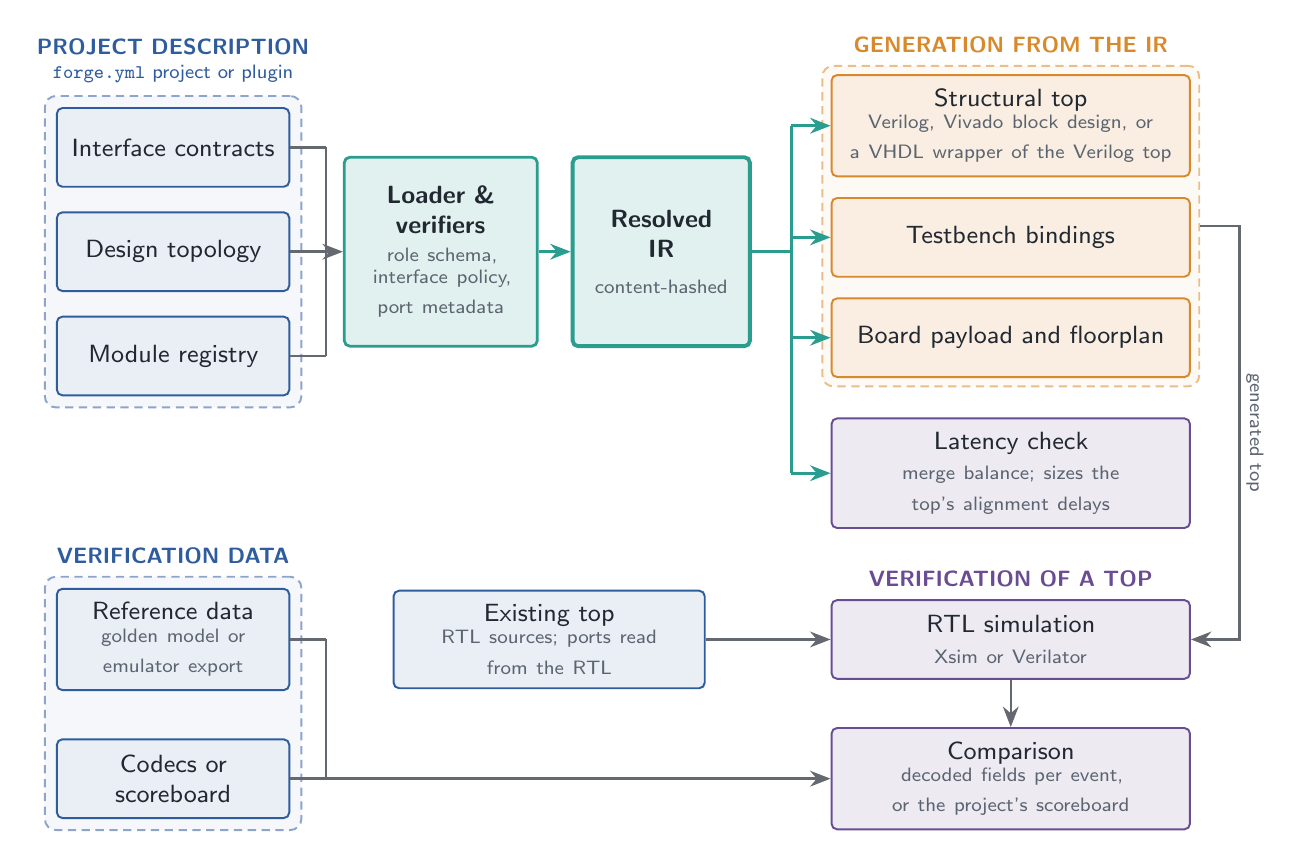
\begin{tikzpicture}
\def\colA{26mm}\def\colD{42mm}

% =============================================================================
% Generation from the IR
% =============================================================================
\node[inbox, text width=\colA] (c1) at (0,0) {Interface contracts};
\node[inbox, text width=\colA, below=3mm of c1] (c2) {Design topology};
\node[inbox, text width=\colA, below=3mm of c2] (c3) {Module registry};

\node[modelbox, text width=21mm, minimum height=24mm] (load) at ($(c2)+(34mm,0)$)
  {\textbf{Loader \&}\\\textbf{verifiers}\\[2pt]
   {\scriptsize\color{subink}role schema,\\interface policy,\\port metadata}};
\node[modelbox, text width=19mm, minimum height=24mm, line width=1.4pt] (ir)
  at ($(load)+(28mm,0)$)
  {\textbf{Resolved}\\\textbf{IR}\\[2pt]{\scriptsize\color{subink}content-hashed}};

\node[genbox, text width=\colD, anchor=west] (g1) at ($(ir.east)+(10mm,16mm)$)
  {Structural top\\{\scriptsize\color{subink}Verilog, Vivado block design, or\\a VHDL wrapper of the Verilog top}};
\node[genbox, text width=\colD, below=2.5mm of g1] (g2)
  {Testbench bindings};
\node[genbox, text width=\colD, below=2.5mm of g2] (g3)
  {Board payload and floorplan};
\node[verbox, text width=\colD, below=5mm of g3] (lat)
  {Latency check\\{\scriptsize\color{subink}merge balance; sizes the top's alignment delays}};

% =============================================================================
% Verification of a top
% =============================================================================
\node[inbox, text width=\colA] (r1) at ($(c3)+(0,-36mm)$)
  {Reference data\\{\scriptsize\color{subink}golden model or\\emulator export}};

\node[inbox, text width=36mm, anchor=west] (ex) at ($(r1.east)+(13mm,0)$)
  {Existing top\\{\scriptsize\color{subink}RTL sources; ports read\\from the RTL}};
\node[verbox, text width=\colD] (sim) at (g1 |- r1)
  {RTL simulation\\{\scriptsize\color{subink}Xsim or Verilator}};
\node[verbox, text width=\colD, below=6mm of sim] (cmp)
  {Comparison\\{\scriptsize\color{subink}decoded fields per event,\\or the project's scoreboard}};
\node[inbox, text width=\colA] (r2) at (r1 |- cmp) {Codecs or scoreboard};

% ---- Groups --------------------------------------------------------------------
\begin{scope}[on background layer]
  \node[groupbg=accInput, fit=(c1)(c3), inner sep=4pt] (gin) {};
  \node[groupbg=accGen, fit=(g1)(g3), inner sep=3pt] (ggen) {};
  \node[groupbg=accInput, fit=(r1)(r2), inner sep=4pt] (gref) {};
\end{scope}
\node[grouptitle=accInput, above=1pt of gin.north, align=center]
  {PROJECT DESCRIPTION\\[-1pt]{\scriptsize\mdseries\texttt{forge.yml} project or plugin}};
\node[grouptitle=accGen, above=1pt of ggen.north] {GENERATION FROM THE IR};
\node[grouptitle=accInput, above=1pt of gref.north] {VERIFICATION DATA};
\node[grouptitle=accVerif, above=1pt of sim.north] {VERIFICATION OF A TOP};

% ---- Flows: generation --------------------------------------------------------
\coordinate (jin) at ($(gin.east)+(3mm,0)$);
\foreach \c in {c1,c2,c3} { \draw[draw=ink!70, line width=0.9pt] (\c.east) -- (jin |- \c); }
\draw[draw=ink!70, line width=0.9pt] (jin |- c1) -- (jin |- c3);
\draw[flow] (jin |- load) -- (load.west);
\draw[flowmodel] (load) -- (ir);

\coordinate (jout) at ($(ir.east)+(5mm,0)$);
\draw[accModel, line width=1.1pt] (ir.east) -- (jout);
\draw[accModel, line width=1.1pt] (jout |- g1) -- (jout |- lat);
\foreach \g in {g1,g2,g3,lat} { \draw[flowmodel] (jout |- \g) -- (\g.west); }

% ---- Flows: verification ------------------------------------------------------
% A generated top and its bindings, or an existing top, are simulated.
\draw[flow] (ggen.east) -- ++(5mm,0) |- node[lbl, pos=0.25, rotate=-90, above]{generated top} (sim.east);
\draw[flow] (ex.east) -- (sim.west);
\coordinate (jref) at ($(gref.east)+(3mm,0)$);
\draw[draw=ink!70, line width=0.9pt] (r1.east) -- (jref |- r1);
\draw[draw=ink!70, line width=0.9pt] (jref |- r1) -- (jref |- r2);
\draw[flow] (r2.east) -- (cmp.west);
\draw[flow] (sim) -- (cmp);

\end{tikzpicture}
\end{document}
